\documentclass[12pt]{article}

\usepackage{fullpage}

\usepackage{geometry}
\geometry{a4paper}

\usepackage{graphicx}
\linespread{1.2}
\usepackage{lmodern}
\usepackage{ragged2e}
\usepackage{amsmath}

\graphicspath{{Img/Lab1/}}

\begin{document}
\begin{titlepage}

\newcommand{\HRule}{\rule{\linewidth}{0.5 mm}}
\center
\textsc{}\\[1cm]
\textsc{\Large Ict for Smart Societies}\\[0.4cm]
\textsc{\large Politecnico di Torino}\\[0.4cm]
\HRule\\[0.5cm]
{\huge \texttt{ICT FOR HEALTH LABORATORY}}\\[0.05cm]
\HRule\\[3cm]

\begin{minipage}{\textwidth}
\large
\emph{Authors:}\\[0.4cm]
\begin{tabular}{lll}
\textsc{Putina} &Andrian & s226673\\
\end{tabular}
\end{minipage}

\vspace{0.7cm}

\begin{minipage}{\textwidth}
\large
\emph{Professor:}\\[0.2cm]
\begin{tabular}{ll}
\textsc{Visentin} &Monica
\end{tabular}
\end{minipage}

\vspace{1cm}

\center {
\includegraphics[scale=0.5]{logo.png}}\\[1cm]

{\large \today}\\[3cm]

\vfill

\end{titlepage}

%------------------------FINE PRIMA PAGINA---------------------------------------

%------------------------SECONDA PAG---------------------------
\tableofcontents
\newpage
%--------------------------------------------------------------

\section{Lab1: Linear Regression \& Parkinson}
The aim of the laboratory is understanding the basic idea of the regression and apply different techniques to obtain the desired results. In particular, it will be considered a database containing a real Parkinson's Disease dataset and different regression solutions will by applied:
\begin{itemize}
\item MSE (Minimum Square Error)
\item Gradient Algorithm
\item Steepest Descent Algorithm
\end{itemize} 
Source: \footnotesize{ https://archive.ics.uci.edu/ml/machine-learning-databases/parkinsons/telemonitoring/}

\subsection{Prepare the Data}
The first script takes as input variable the total number of pacients \texttt{Npacients} and converts the fourth column (test\_time) into its integer part.
Furthermore creates a new matrix containing, for all the dates, only the mean of the measurements for each pacient so at the end the new matrix has one row for each day (with the mean of the measured values of the features) for each pacient.

\begingroup
    \fontsize{12pt}{8pt}\selectfont
\begin{verbatim}
close all
clear all
%Lab 1 - ICT HEALTH - Prepare the data

load('updrs.mat');

Npacients = 42;
parkinsonsupdrs(:,4) = abs(floor(parkinsonsupdrs(:,4)));

finalMatrix = [];
for pacient = 1: Npacients

    rowPacient = parkinsonsupdrs(:, 1) == pacient;
    matrixPacient = parkinsonsupdrs(rowPacient,:);

    count = 0;
    for day = 1:max(parkinsonsupdrs(:,4))+1
       indx = matrixPacient(:,4) == day-1;
       if (any(indx(:) == 1))
           count = count+1;
           meanMatrixPacient(count,:) = mean(matrixPacient(indx,:));
       end
    end

    finalMatrix = [finalMatrix; meanMatrixPacient];
    meanMatrixPacient=[];

end
save('finalMatrix','finalMatrix');
\end{verbatim}
\endgroup
The next step is to divide the pacients into two groups. The first sub-group will be used for the training phase of the algorithm while the second one will be used for the testing part. Anyway the data has to have zero mean and variance equal to 1 (EXPLAIN WHY!!!). The easiest way is to subscract the mean of each feature  
to all the pacients and divide by the standard deviation. Obviously the mean and the standard deviation is computed on training data we decided before. The data is now normalized so has zero mean and variance = 1

\begingroup
	\fontsize{12pt}{8pt}\selectfont

    \begin{verbatim}
close all
clear all
%Lab 1 - ICT HEALTH - Prepare data for train

load('finalMatrix.mat');

Npacients = 36;
rowPacients_train = finalMatrix(:,1) <= Npacients;
rowPacients_test =  finalMatrix(:,1) > Npacients;

data_train = finalMatrix(rowPacients_train,:);
    m_data_train = mean(data_train,1);
    v_data_train = var(data_train,1);
    std_data_train = std(data_train,1);

    data_train_norm = data_train(:,5:22) - m_data_train(:,5:22);
    data_train_norm = data_train_norm ./ std_data_train(:,5:22);
    data_train_norm = [data_train(:,1:4), data_train_norm];

data_test = finalMatrix(rowPacients_test,:);
    data_test_norm = data_test(:,5:22) - m_data_train(:,5:22);
    data_test_norm = data_test_norm ./ std_data_train(:,5:22);
    data_test_norm = [data_test(:,1:4), data_test_norm];

save('data_train_norm','data_train_norm');
save('data_test_norm','data_test_norm');
\end{verbatim}

\endgroup

\subsection{Perform Regression with MSE}
QUALCOSA DI SCRITTO SULLA TEORIA

\begingroup
	\fontsize{12pt}{8pt}\selectfont

    \begin{verbatim}
close all
clear all
%Lab 1 - ICT HEALTH - Perform regression - MSE

load('data_train_norm.mat');
load('data_test_norm.mat');

F0 = 7;
flag_features = 4; %first features

y_train = data_train_norm(:,F0);
y_test = data_test_norm(:,F0);

X_train = data_train_norm(:,flag_features:end);
X_test = data_test_norm(:,flag_features:end);
X_train(:,F0-flag_features) = [];
X_test(:,F0-flag_features)=[];

% Estimate a_hat
a_hat = inv(transpose(X_train)*X_train)*transpose(X_train)*y_train;
y_hat_train = X_train * a_hat;
y_hat_test = X_test * a_hat;

figure
plot(y_hat_train)
hold on
plot(y_train, '--k')
axis([0 840 -2 18])
grid on
legend('y\_hat\_train','y\_train', 'Location', 'northwest')
title('y\_hat\_train vs y\_train')

figure
plot(y_test)
hold on
plot(y_hat_test, '--k')
axis([0 150 -1.75 3.5])
grid on
legend('y\_hat\_test','y\_test')
title('y\_hat\_test vs y\_test')

figure
hist(y_hat_train - y_train, 50)
grid on

figure
hist(y_hat_test - y_test, 50)
grid on
\end{verbatim}
\endgroup
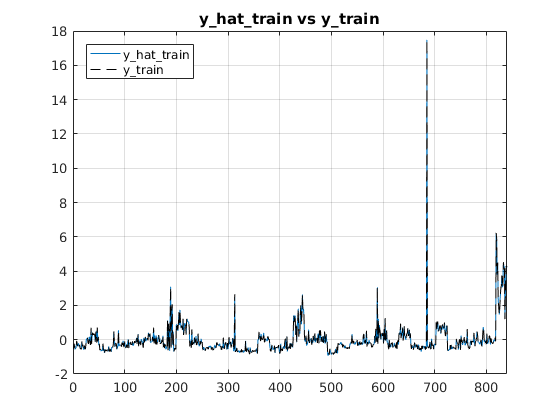
\includegraphics [width=3in]{Lab1Part3_01.png}
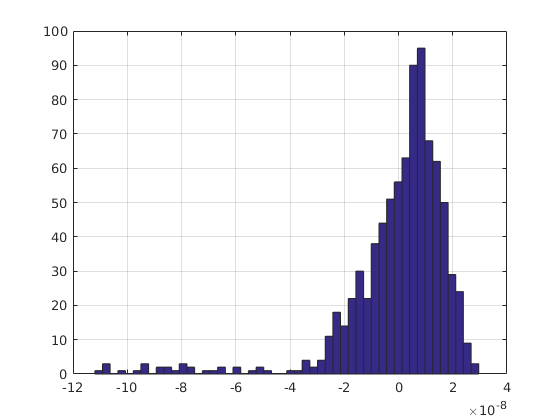
\includegraphics [width=3in]{Lab1Part3_03.png}

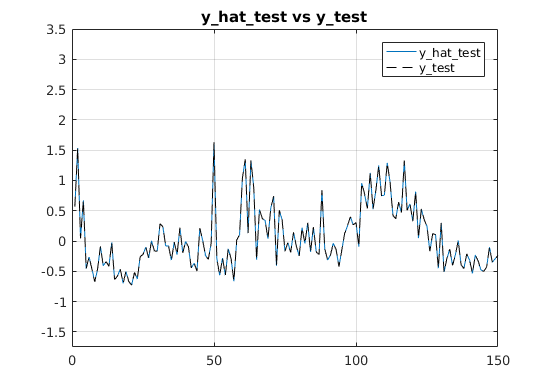
\includegraphics [width=3in]{Lab1Part3_02.png}
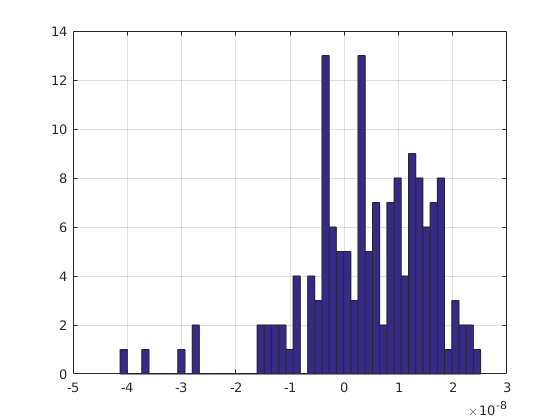
\includegraphics [width=3in]{Lab1Part3_04.png}






\end{document}